\documentclass{article}

\usepackage{amsmath}
\usepackage{amssymb}
\usepackage{bbold}
\usepackage[makeroom]{cancel}
\usepackage[margin=1in]{geometry}
\usepackage{graphicx}
\usepackage{hanging}
\usepackage{hyperref}
\usepackage[parfill]{parskip}

\setlength\parindent{0pt}
\renewcommand{\baselinestretch}{1.5}

\frenchspacing

\title{Ninnion: The Observer's Operation Manual}
\author{Cristina Torres Memorial Observatory \\
	Brownsville, Texas}
\date{v 7 Sep 2023}

% Initial version: 3 Jul 2019

\begin{document}
	
	\maketitle
	
	\begin{figure}[b]
		\centering
		\includegraphics[scale=0.2]{images/CTMO_transparent.png}
	\end{figure}
	
	\newpage
	\tableofcontents
	
	\newpage
	\section{Planning an Observation}
	\label{sec:planning-an-observation}
	
	Planning an observation requires a few critical steps that should be completed before arriving at the observatory. Entering the observatory with an observation strategy and understanding of the sky conditions is crucial for completing a scientific observation.
	
	\subsection{Check the weather and sky conditions}
	\label{sec:check-the-weather-and-sky-conditions}
	
	\begin{enumerate}
		
		\item Check sunset. It is advised that you choose the beginning of your critical scientific data run to be no earlier than astronomical twilight. Astronomical twilight occurs when the Sun is 18 degrees below the local horizon. In Brownsville, during the summer, astronomical twilight occurs roughly 1.5 hours after sunset. You can certainly observe before this time, during civil or nautical twilight, but extinction by sunlight will be much more significant. See Figure \ref{fig:twilight}.
		
		\item Check forecast. Visit the \href{https://www.weather.gov}{National Weather Service}. See Figure \ref{fig:nws}.
		
		\begin{enumerate}
			
			\item At the top left, search and select the location \texttt{Olmito, TX, USA}. This action will take you to a new page with the forecast for Olmito.		
			
			\item Scroll down the new page to the section titled \texttt{Detailed Forecast}. See Figure \ref{fig:forecast}.
			
			\item To the right of this you will see a map. There will be a green square on the map already, but ignore it for now. Find the approximate location of the observatory and click it on the map. Wait for the page to reload. You should see the green square highlighting the region you just clicked. See Figure \ref{fig:position}.
			
			\item Immediately below this, click the graph titled \texttt{Hourly Weather Forecast}. This action takes you to a new page with the forecast in graphical form of the location you clicked. See Figure \ref{fig:graphical}. This page is extremely useful and it is recommended to bookmark this page for future reference. You will want to monitor the changing conditions throughout the day before your observation. Typically, 50\% or greater cloud coverage is a sign that an observation is a no-go.
			
		\end{enumerate}
		
		\item Check the Moon. Using Stellarium, check to see the phase and position of the Moon during the course of the night. Moonlight significantly interferes with photometric precision. You'll want to make sure your targets are far enough away from the Moon so as not to affect your exposures.
		
	\end{enumerate}
	
	\subsection{Identify your target}
	\label{sec:identify-your-target}
	
	\begin{enumerate}
		
		\item What are the coordinates of your object? Object coordinates are typically expressed in right ascension (\texttt{hh:mm:ss.ssss}) and declination (\texttt{$\pm$dd:mm:ss.ssss}) in the J2000 epoch.
		
		\item Check the altitude range over your expected observation time. For accurate photometry, you want to make sure your object is above 30 degrees in altitude. It is useful to visualize the path of the object in the sky ahead of time, using planetarium software like Stellarium.
		
		\item Obtain a reference field for your night. Using software such as Stellarium, or any optical image database online like \href{http://simbad.u-strasbg.fr/simbad/}{SIMBAD} or the \href{https://archive.stsci.edu/cgi-bin/dss_form}{STScI Digitized Sky Survey}. Finding archival images of your target fields will also help you check the pointing of the telescope.
		
		\item Determine suitable reference stars. Make sure they are not variable stars and that their color indices are similar to your target object.
		
	\end{enumerate}
	
	\subsection{Plan your observing strategy}
	\label{sec:plan-your-observing-strategy}
	
	\begin{enumerate}
		
		\item What is your strategy?
		
		\begin{enumerate}
			
			\item Do you have a list of targets that you want to observe throughout the night?
			
			\item Are you tracking a single object?
			
			\item Does the object have significant proper motion?
			
		\end{enumerate}
		
		\item If you plan to observe multiple objects, like a selection of galaxies, then you want to observe the targets that are scheduled to set first. That way you can observe the most amount of galaxies on your list at a suitable air mass.
		
		\item If you plan to observe a single target over time, then you will need to decide on the exposure time and cadence of your image sequence. This answer will depend on the nature of your target and the response of the optical system.
		
		\begin{enumerate}
			
			\item Asteroids move with proper motion and can have a wide range of velocities.
			
			\item Exoplanet transits can be quite faint and are at a fixed point in time.
			
			\item Variable stars have a wide variety of periods and magnitude changes.
			
			\item Filters, a significant Moon, and low altitude are examples of factors that reduce the signal-to-noise ratio (SNR) and change the color of your target.
			
		\end{enumerate}
		
	\end{enumerate}
	
	\newpage
	\section{Starting Up}
	\label{sec:starting-up}
	
	\subsection{Entry and power up}
	\label{sec:entry-and-power-up}
	
	\begin{enumerate}
		
		\item Remove padlocks from the hatch. Bring padlocks inside.
		
		\item Turn on the lights. Use the switch on the right side entering the dome.
		
		\item Bring the padlocks and your personal belongings into the control room. Remember that the control room door should always be shut.
		
		\item Message the team on the ``CTMO Leaders'' WhatsApp group that the dome has been opened.
		
		\item Turn on all circuit breakers 1-12. Breakers numbered 2, 5, 7, and 11 should always remain on.
		
		\item Turn on the UPS battery backup. This is the slim, tall box on the table to the immediate left of the breaker box. Turn it on using the center power button. After a beep and some warming up, the information screen should indicate the battery is running on the power line rather than on the battery.
		
		\item In the control room, turn on the A/C unit using the black remote mounted on the wall. The A/C unit works as both an air conditioner and a heater. Press the \texttt{Mode} button on the remote, and you will be able to see on the left side of the display that the remote is cycling through its settings. The heater light will display red on the A/C unit as confirmation if you chose the heater mode. You adjust the temperature regardless of mode by clicking the up and down buttons on the remote. Note: For the heater, it will not kick on immediately. Give the heater about five minutes to warm up.
		
		\item Turn on Atlas. First, you need to toggle the power switch on the back of the computer. GRUB should automatically boot Windows.
		
	\end{enumerate}
	
	\subsection{Open shutter window}
	\label{sec:open-shutter-window}
	
	\begin{enumerate}
		
		\item Unplug the battery charger from the wall outlet.
		
		\item Remove the charger from the battery. First remove the red leads from the red (+) terminal on the battery. Then remove the black lead from the black (-) terminal on the battery.
		
		\item Remove the charger from the wall and place it safely on the floor.
		
		\item Take the shutter controller with the plastic cover. Press the green power button on the controller. Press and hold \texttt{UP} on the shutter controller. Open until the white rubber lip of the shutter window is coincident with the blue metal bar near zenith.
		
	\end{enumerate}
	
	\subsection{Open shutter door}
	\label{sec:open-shutter-door}
	
	\begin{enumerate}
		
		\item Undo the rope and let down the shutter door. It is normal for the rope to stretch diagonally across the shutter door opening.
		
	\end{enumerate}
	
	\subsection{Prepare telescope}
	\label{sec:prepare-telescope}
	
	\begin{enumerate}
		
		\item Slide the light shroud up toward the front of the optical tube assembly (OTA).
		
		\item Remove the cloth cover from the secondary mirror.
		
		\item Remove the plastic shower cap.
		
		\item Remove the round plastic lid from the primary aperture.
		
		\item Slide the light shroud back down to completely enclose the OTA.
		
		\item Turn on the mount.
		
		\item Make sure all cables attached to the telescope and accessories are loose and that there is enough free cable to allow for the telescope's full range of motion.
		
	\end{enumerate}
	
	\subsection{Connect to EFA kit}
	\label{sec:connect-to-efa-kit}
	
	\begin{enumerate}
		
		\item Open PWI3. Verify the computer established connection to the electronic focus assembly (EFA). The EFA should connect automatically to the computer and begin cooling the OTA and primary mirror. You should hear the fans in the mount turn on.
		
		\item Click the \texttt{Temperature} tab on the right in PWI3. Record the ambient temperature given by the display.
		
	\end{enumerate}
	
	\subsection{Connect to camera}
	\label{sec:connect-to-camera}
	
	\begin{enumerate}
		
		\item Open MaxIm DL.
		
		\item Connect to the camera. Under \texttt{View}, open the \texttt{Camera Control Window}. Select \texttt{Setup} and then \texttt{Connect} to enable computer connection to the camera.
		
		\item Cool the camera. Click \texttt{Cooler} and enter the set point. It is advisable to limit the initial set point to no more than 40 degrees C relative to the ambient temperature to avoid over-straining the thermoelectric coolers. For example, if the ambient temperature is 30 degrees C, then the set point should be about -10 degrees C.
		
		\item Under \texttt{Connect} select \texttt{On} to begin cooling the camera. The cooler power should not exceed 80\% during stable operation (although the power might exceed this during the cooling phase).
		
		\item Once the camera temperature stabilizes, take 10 bias frames on \texttt{Continuous} (these don't need to be saved). Taking a quick set of bias frames will clear any residual charge stored from previous exposures on the CCD.
		
	\end{enumerate}

	\subsection{Connect to filter wheel}
	\label{sec:connect-to-filter-wheel}
	
	\begin{enumerate}
		
		\item Open FLIFilter. Click \texttt{Home}.
		
		\item The filter wheel will initially be at position ``unknown'' and will end up at slot 0 ``unfiltered''. You can select filters by clicking each of their corresponding buttons once homing is finished.
		
		\item If you click \texttt{CW} or \texttt{CCW}, you will have to re-home the filter wheel before selecting another one.
		
		\item You might have to manually jog the filter wheel after selecting a new filter by using the \texttt{CW} or \texttt{CCW} buttons. Make sure to re-home the filter wheel before selecting another filter.
		
	\end{enumerate}
	
	\subsection{Connect to mount}
	\label{sec:connect-to-mount}
	
	\begin{enumerate}
		
		\item Open PWI4. Click \texttt{Connect} at the top left of the window.
		
		\item Click \texttt{Enable RA} and \texttt{Enable Dec} under \texttt{Connect}.
		
		\item Make sure the area around the telescope is completely clear. Select \texttt{Commands} and then click \texttt{Home Mount}. The telescope will slew and locate its reference encoders.
		
		\item Once the telescope has stopped moving, you are ready to observe!
		
	\end{enumerate}
	
	\newpage
	\section{Observing}
	\label{sec:observing}
	
	\subsection{Slew telescope}
	\label{sec:slew-telescope}
	
	\begin{enumerate}
		
		\item In PWI4, under the \texttt{Goto} tab, enter the right ascension and declination of your intended object. Make sure the format is either sexagesimal (\texttt{hh:mm:ss.ssss} and \texttt{$\pm$dd:mm:ss.ssss}) or decimal (\texttt{dd.dddd} and \texttt{$\pm$dd.dddd}).
		
	\end{enumerate}

	\subsection{Rotate dome}
	\label{sec:rotate-dome}
	
	\begin{enumerate}
		
		\item Using the uncovered remote, press the \texttt{West} button to rotate the dome window to the desired position. Due to current limitations with the dome, the \texttt{East} button should not be used.
		
	\end{enumerate}
	
	\subsection{Take test exposure}
	\label{sec:take-test-exposure}
	
	\begin{enumerate}
		
		\item In MaxIm DL, under the \texttt{Expose} tab, select a ``Single'' exposure (under the \texttt{Start} button on the right).
		
		\item Enter an exposure time under \texttt{Seconds}.
		
		\item Subframes should be disabled, unless you're doing an observation that specifically needs them.
		
		\item Select the binning under the \texttt{X Binning} drop-down list. Binning should match the nightly atmospheric seeing, as well as chosen for balancing the SNR and resolution of your particular object. Higher binning means higher SNR per pixel, but at a loss of pixel resolution on the overall image.
		
		\item If your image is out of focus, go to the \texttt{AF CONFIG} tab in PWI3. Take an image count (\texttt{Steps}) of 10 and set the exposure length (under \texttt{Seconds}) and binning (under \texttt{X Binning}) you will be using for your target. Under the tab \texttt{AF CONFIG}, click \texttt{START AF}, which will focus your images. Wait until all 10 images are done being processed.
		
		\item Additionally, in the \texttt{Options} menu, make sure that dark frames are not being automatically subtracted.
		
		\item Finally, once your telescope is settled on a target and your exposure parameters are set, click the \texttt{Start} button at the top right of the camera control window. The idle bar will begin to fill as the exposure commences. A picture should automatically render in MaxIm DL once the exposure is complete. First light!
		
		\item If you used ASCOM (see \hyperref[sec:set-up-ascom]{Appendix A}), to test the ASCOM connection, to go \texttt{View}, select \texttt{FITS Header Window}, and check for \texttt{EXPTIME}, \texttt{FOCUSPOS}, \texttt{OBJCTRA}, and \texttt{OBJCTDEC} to make sure it is reading the correct information you are using with your observation. 
		
	\end{enumerate}
	
	\subsection{Set up directory structure}
	\label{sec:set-up-directory-structure}
	
	\begin{enumerate}
		
		\item Under \texttt{C:\textbackslash Documents\textbackslash Observations} create a directory with the evening date in the format \texttt{yyyy-mm-dd}.
		
		\item Under the newly-made directory, create a directory called \texttt{dark}, a directory called \texttt{flat}, and a directory for each of your targets by name (e.g. for target exoplanet system HAT-P-7 the directory would be something like \texttt{hatp7}). See Figure~\ref{fig:directory}.
		
	\end{enumerate}
	
	\subsection{Set up autosave routine}
	\label{sec:set-up-autosave-routine}
	
	Note that if you choose multiple targets, you can either i) set up multiple autosave routines, or ii) use the \texttt{Single} exposure option to manually expose each target.
	
	\begin{enumerate}
		
		\item In MaxIm DL, in the \texttt{Camera Control} window, under the \texttt{Expose} tab, click the \texttt{Autosave} button. A new window should appear called \texttt{Autosave Setup}.
		
		\item In the \texttt{Autosave Setup} window, set \texttt{Autosave Filename} to the name of your target.
		
		\item Make sure \texttt{Slot 1} is selected. Frame \texttt{Type} will be \texttt{Light}. Set your \texttt{Exposure}, \texttt{Binning}, and the number of exposures or \texttt{Repeat}.
		
		\item Select \texttt{Options} and \texttt{Set Image Save Path...}. Under \texttt{Documents}, \texttt{Observations}, create a new directory with the current date (in \texttt{yyyy-mm-dd} format). Then, under this new directory, create a new subdirectory with the name of your target. Click \texttt{OK} to close this window.
		
		\item Finally, in the \texttt{Autosave Setup} window, select \texttt{Apply} followed by \texttt{OK} to close the window.
		
		\item In the \texttt{Camera Control} window, select \texttt{Start} to begin taking data.
		
	\end{enumerate}

	\subsection{Set up observer log}
	\label{sec:set-up-observer-log}
	
	\begin{enumerate}
		
		\item In a web browser, navigate to the \href{https://forms.office.com/pages/responsepage.aspx?id=pjYEmd-HHEmRJJr6kfiIJ6_-JTSTSFFHivQ4LTyBzxRUNjk5SEFNSkY1QzA2UlMwVUdUR1ROUVpCSS4u}{Observer's Journal}.
		
		\item Create a new entry and submit a completed form by the end of the observation.
		
	\end{enumerate}
	
	\subsection{Monitor observing conditions}
	\label{sec:monitor-observing-conditions}
	
	\begin{enumerate}
		
		\item Weather and sky coverage should be a priority, since this directly affects the data stream and could pose risks to the telescope and dome.
		
		\item Make sure the dome shutter window remains in line with the telescope pointing. At the time of writing, the dome rotation has not been integrated into the telescope motion.
		
		\item Make sure the data is being saved in the correct directory and recorded in the data log.
		
	\end{enumerate}
	
	\subsection{Take calibration frames}
	\label{sec:take-calibration-frames}
	
	\subsubsection{Flat frames}
	\label{sec:flat-frames}
	
	\begin{enumerate}
		
		\item Make sure the area around the telescope is completely clear.
		
		\item In PWI4, select \texttt{Commands} and then click \texttt{Home Mount}. The telescope will slew and locate its reference encoders.
		
		\item In PWI4, under the \texttt{Goto} tab, enter the right altitude and azimuth of the flatfield screen. Use an azimuth of 352 degrees and an altitude of 12 degrees. You will then need to slew the dome to center the flatfield screen in the telescope FOV.
		
		\item Connect the dimmer switch plug and press the dimmer switch knob to click it on. Next, turn the dimmer switch to produce some light and take a test exposure. This process will be iterative until the appropriate level is reached. The average pixel value across the frame should be roughly 50\% the saturation limit of the camera. For a 16-bit camera like the ProLine 16803, the saturation limit is 65535 counts.
		
		\item Take a series of at least 15 flats per filter used that night.
		
	\end{enumerate}

	\subsubsection{Dark frames}
	\label{sec:dark-frames}
	
	\begin{enumerate}
		
		\item Turn off lights and take a series of 15 dark frames. For each integration time used in an observation (including those of your flats), a series of 15 darks per integration time will be needed.
		
	\end{enumerate}
	
	\newpage
	\section{Shutting Down}
	\label{sec:shutting-down}
	
	\subsection{Disconnect from mount}
	\label{sec:disconnect-from-mount}
	
	\begin{enumerate}
		
		\item Make sure the area around the telescope is completely clear.
		
		\item In PWI4, select \texttt{Commands} and then click \texttt{Home Mount}. The telescope will slew and locate its reference encoders.
		
		\item Close PWI4.
		
		\item If you used ASCOM (see \hyperref[sec:set-up-ascom]{Appendix A}), disconnect \texttt{Telescope}, \texttt{Dome}, and \texttt{Focuser}. Close ASCOM.
		
	\end{enumerate}

	\subsection{Disconnect from EFA kit}
	
	\begin{enumerate}
	
		\item In PWI3, select \texttt{Disconnect} at the top right of the window to turn off the OTA fans.
		
		\item Close PWI3.
		
	\end{enumerate}

	\subsection{Disconnect from filter wheel}
	\label{sec:disconnect-from-filter-wheel}
	
	\begin{enumerate}
		
		\item Home the filter wheel.
				
		\item Close FLIFilter.
		
	\end{enumerate}
	
	\subsection{Disconnect from camera}
	\label{sec:disconnect-from-camera}
	
	\begin{enumerate}
		
		\item In MaxIm DL, in the \texttt{Camera Control Window}, select \texttt{Setup} and then \texttt{Warm Up} to begin warming up the camera.
		
		\item Wait until the cooler power has dropped to close to 0\% and the temperature of the chip is close to the ambient temperature. This might take a while, therefore you may continue with shutting down the rest of the observatory (up to, but not including, turning off the UPS battery backup) and then come back to this point.
		
		\item Select \texttt{Off} under \texttt{Setup} to turn off the camera cooler.
		
		\item Select \texttt{Disconnect} and then close MaxIm DL.
		
		\item Shut down the computer (allow for updates before shutting off power). Turn off the monitors.
		
	\end{enumerate}
	
	\subsection{Cover telescope}
	\label{sec:cover-telescope}
	
	\begin{enumerate}
		
		\item Turn off the mount.
		
		\item Slide the light shroud up toward the front of the OTA.
		
		\item Replace the round plastic lid onto the primary aperture.
		
		\item Replace the plastic shower cap and use clips to fasten it.
		
		\item Replace the cloth cover onto the secondary mirror.
		
		\item Slide the light shroud back down to completely enclose the OTA.
		
	\end{enumerate}
	
	\subsection{Close shutter door}
	\label{sec:close-shutter-door}
	
	\begin{enumerate}
		
		\item Pull the door back up to its original position.
		
		\item Wrap the rope completely around the handle, making sure the door remains flush against the dome (even with a decent push). Tie the rope into a knot to keep it secure.
		
	\end{enumerate}
	
	\subsection{Close shutter window}
	\label{sec:close-shutter-window}
	
	\begin{enumerate}
		
		\item Press and hold \texttt{CLOSE} on the shutter controller (the one with a plastic cover). Close the shutter until the shutter door automatically stops.

		\item Place the charger on the wall. Connect the charger to the battery.
		
		\item First connect the BLACK lead to the BLACK (-) terminal on the battery. Then connect the RED lead to the RED (-) terminal on the battery.
		
	\end{enumerate}
	
	\subsection{Power down and exit}
	\label{sec:power-down-and-exit}
	
	\begin{enumerate}
		
		\item Turn off the AC unit in the control room.
		
		\item Turn off the UPS battery backup. Press and hold the center power button until you hear it beep.
		
		\item Turn off circuits breakers. Breakers 2, 5, 7, and 11 should always remain ON.
		
		\item Turn off the lights, both inside and outside the control room, and shut the control room door.
		
		\item Exit the dome and replace the padlocks on the hatch.
		
		\item Message the team that the dome has been closed.
		
	\end{enumerate}

	\newpage

	\newpage
	\appendix
	
	\section{Set up ASCOM}
	\label{sec:set-up-ascom}
	
	\begin{enumerate}
		
		\item Open ASCOM Device Hub. Click \texttt{Device Setup} and click \texttt{Tools}.
		
		\item Click \texttt{Telescope Setup}, click \texttt{Choose}, select \texttt{Plane Wave Interface}, click \texttt{OK}.
		
		\item Click \texttt{Dome Setup}, click \texttt{Choose}, select \texttt{Dome Simulator NET}, click \texttt{OK}. 
		
		\item Click \texttt{Focuser Setup}, click \texttt{Choose}, select \texttt{PlaneWave Focuser PWI3}, click \texttt{OK}. 
		
		\item Connect \texttt{Telescope} to \texttt{Device HUB}. 
		
		\item Connect \texttt{HUB} to \texttt{Device HUB}. 
		
		\item Connect \texttt{Focuser} to \texttt{Device HUB}. 
		
		\item Open MaxIm DL Pro 5. At the top click \texttt{View} and then go to \texttt{Observatory Control Window}. 
		
		\item Under \texttt{Telescope}, click \texttt{Options}, click \texttt{Choose}, select \texttt{Device Hub Telescope}, click \texttt{OK}. 
		
		\item Next, under \texttt{Dome}, click \texttt{Options}, click \texttt{Choose}, select \texttt{Device Hub Dome}, click \texttt{OK}. 
		
		\item Next, go to \texttt{Focuser 1}, click \texttt{Choose}, select \texttt{Device Hub Focuser}, then click \texttt{OK}. 
		
		\item At the very bottom, click \texttt{Option} and \texttt{Connect All}. 
		
		\item You can compare the right ascension and declination of the telescope pointing given by MaxIM to that given by PWI4. 
		
		\item Next, you will click on \texttt{Dome}, go to \texttt{Options}, click \texttt{Slewing Parameters}.
		
		\item Here we can compare the focuser position given by MaxIM DL to that given by PWI3. Focusing corrections can be made by reading the MaxIm position and moving the focus status position in PWI3.
		
		\item Go to \hyperref[sec:take-test-exposure]{Section 3.3, Step 8} to test if ASCOM is running. 
		
	\end{enumerate}	
	
	\newpage
	\section{Figures}
	\label{sec:figures}
	
	\begin{figure}[htbp!]
		\centering
		\includegraphics[scale=0.5]{images/twilight-phases-dusk.png}
		\caption{The definition of dusk (or twilight) depending on the altitude of the Sun below the local horizon.}
		\label{fig:twilight}
	\end{figure}

	\begin{figure}[htbp!]
		\centering
		\includegraphics[scale=0.3]{images/nws.png}
		\caption{The home page of the National Weather Service.}
		\label{fig:nws}
	\end{figure}

	\begin{figure}[htbp!]
		\centering
		\includegraphics[scale=0.3]{images/detailed_forecast.png}
		\caption{The detailed forecast of the default location selected for Olmito, TX.}
		\label{fig:forecast}
	\end{figure}

	\begin{figure}[htbp!]
		\centering
		\includegraphics[scale=0.5]{images/green_square.png}
		\caption{The green square after the page reloads, indicating the correct position has been selected.}
		\label{fig:position}
	\end{figure}

	\begin{figure}[htbp!]
		\centering
		\includegraphics[scale=0.5]{images/graph.png}
		\caption{The graphical forecast at the location of the observatory.}
		\label{fig:graphical}
	\end{figure}

	\begin{figure}[htbp!]
		\centering
		\includegraphics[angle=270, scale=0.05]{images/circuits.png}
		\caption{The circuit breaker with panel open and switches revealed. Note that all circuits are switched on for operating the observatory. Circuits 2, 5, 7, and 11 remain switched on even after closing.}
		\label{fig:circuits}
	\end{figure}

	\begin{figure}[htbp!]
		\centering
		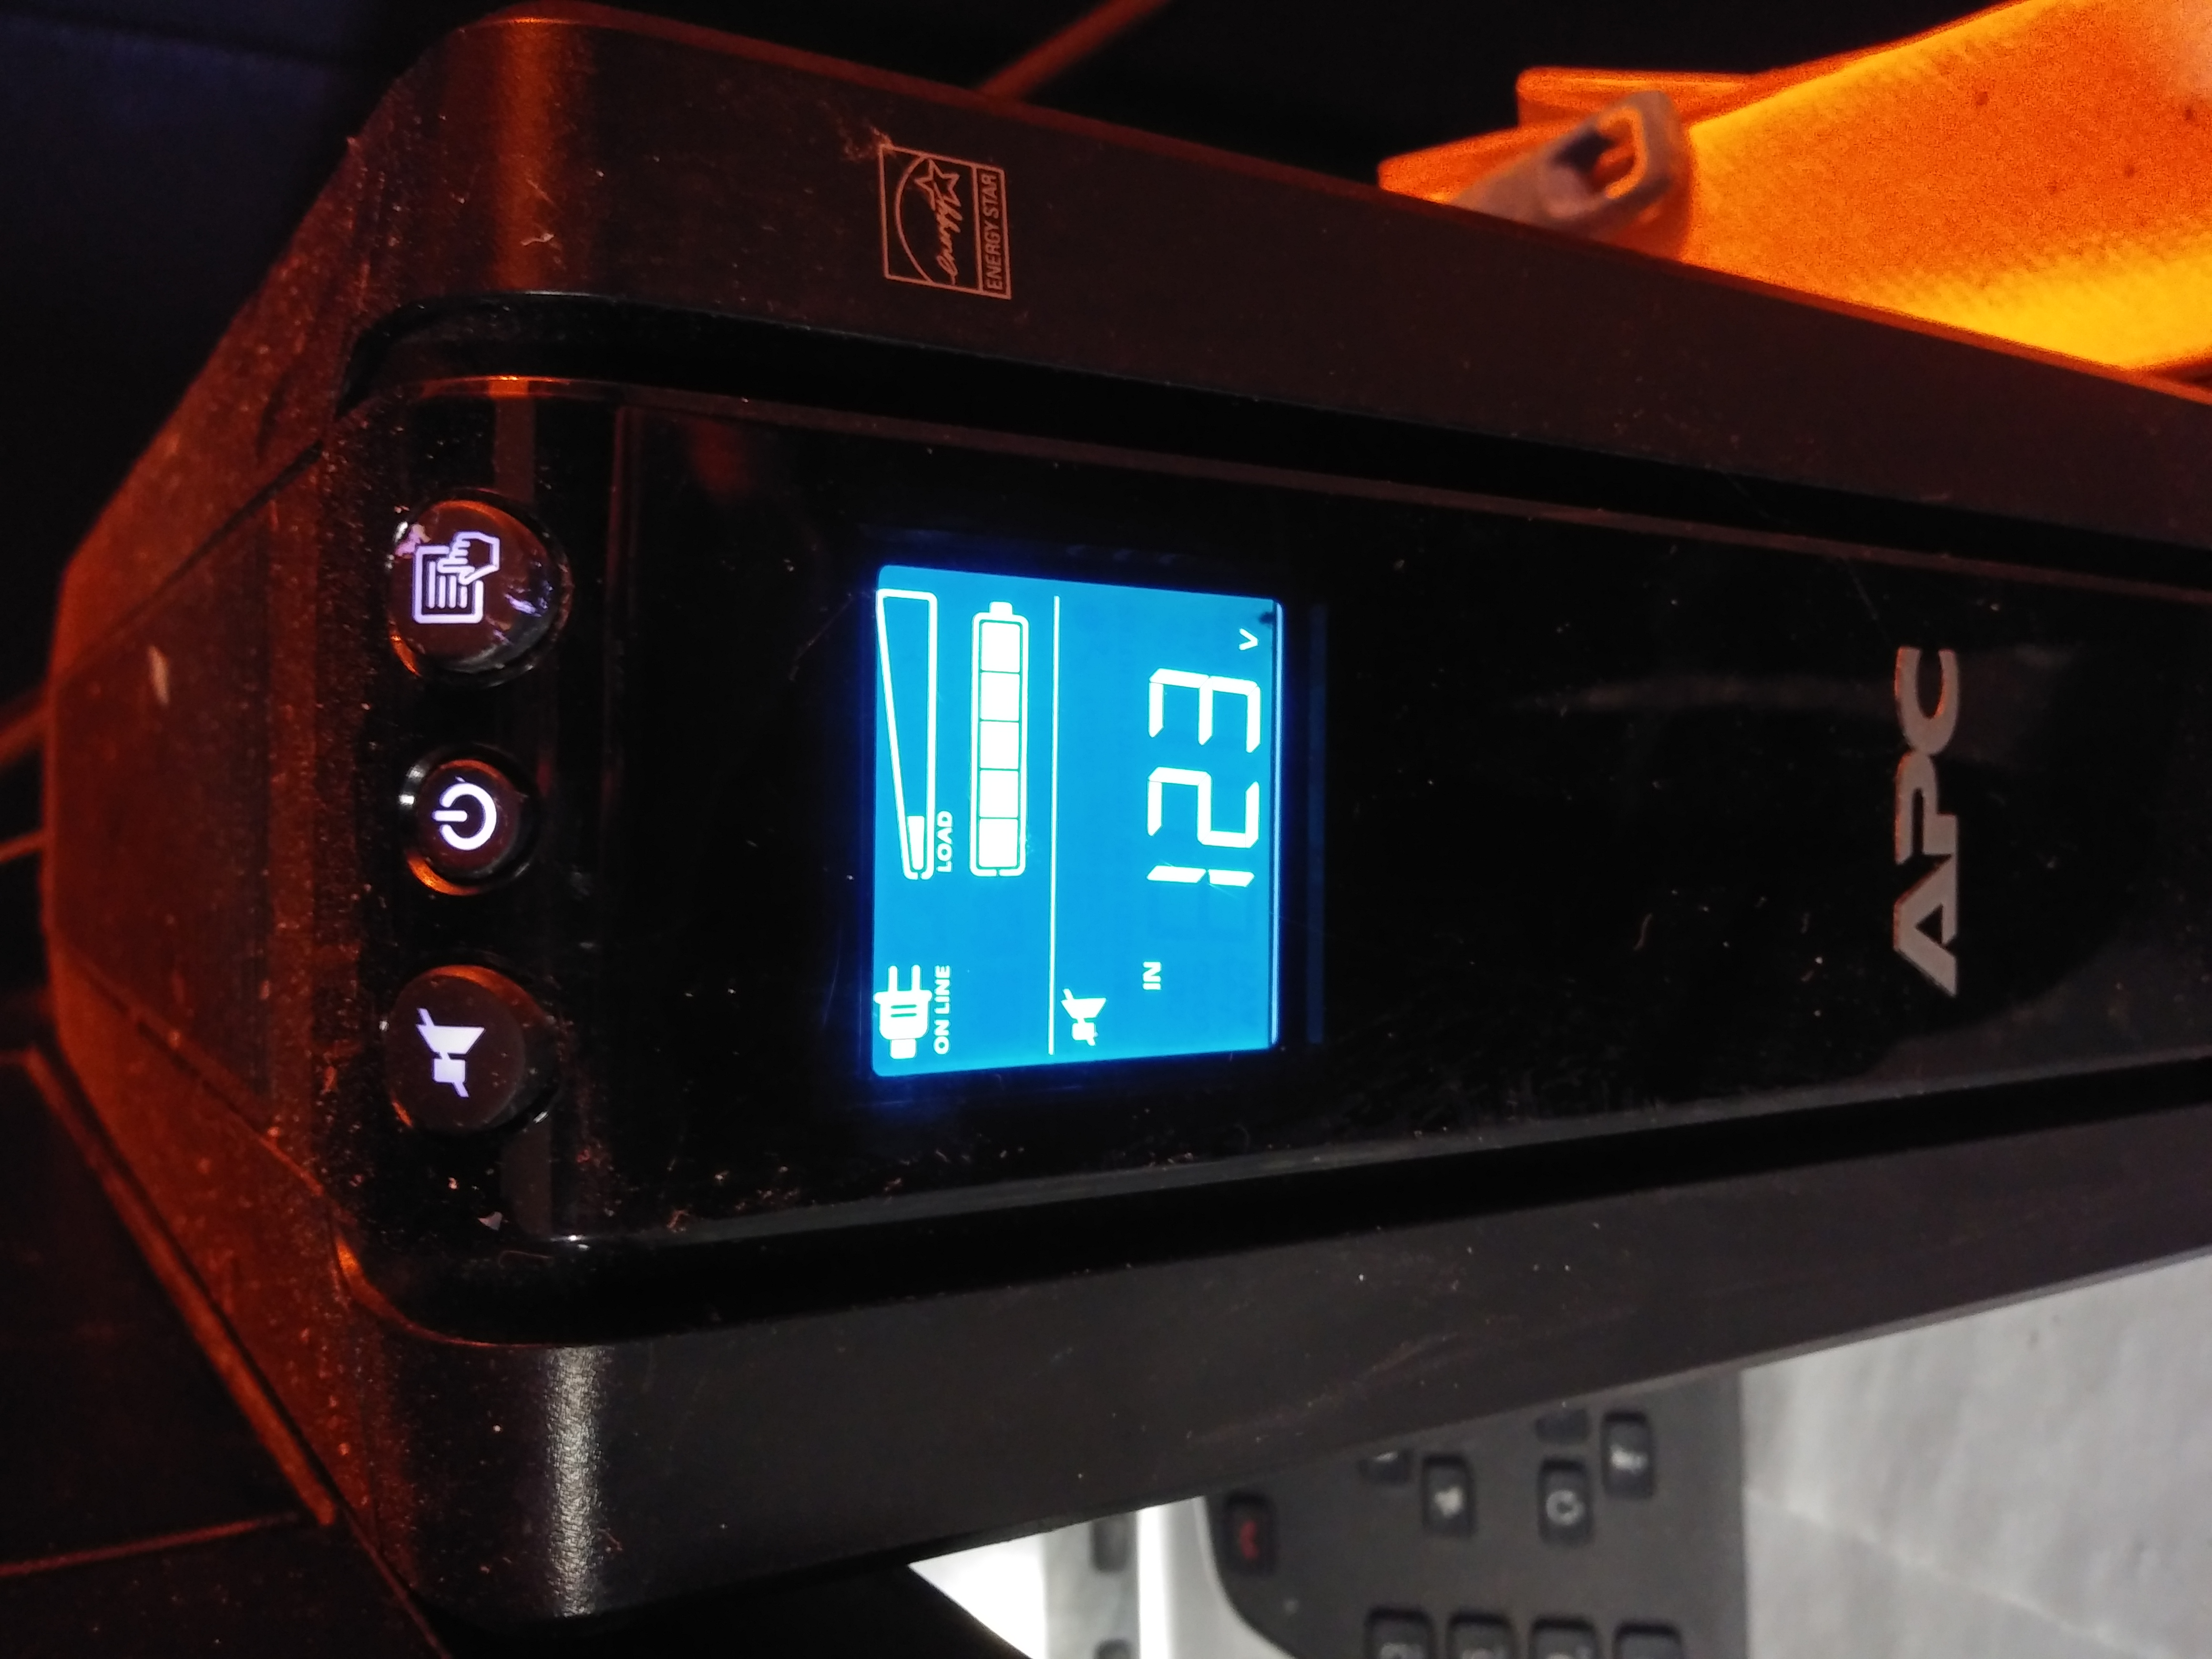
\includegraphics[angle=270, scale=0.05]{images/ups_backup.png}
		\caption{Caption.}
		\label{fig:ups}
	\end{figure}

	\begin{figure}[htbp!]
		\centering
		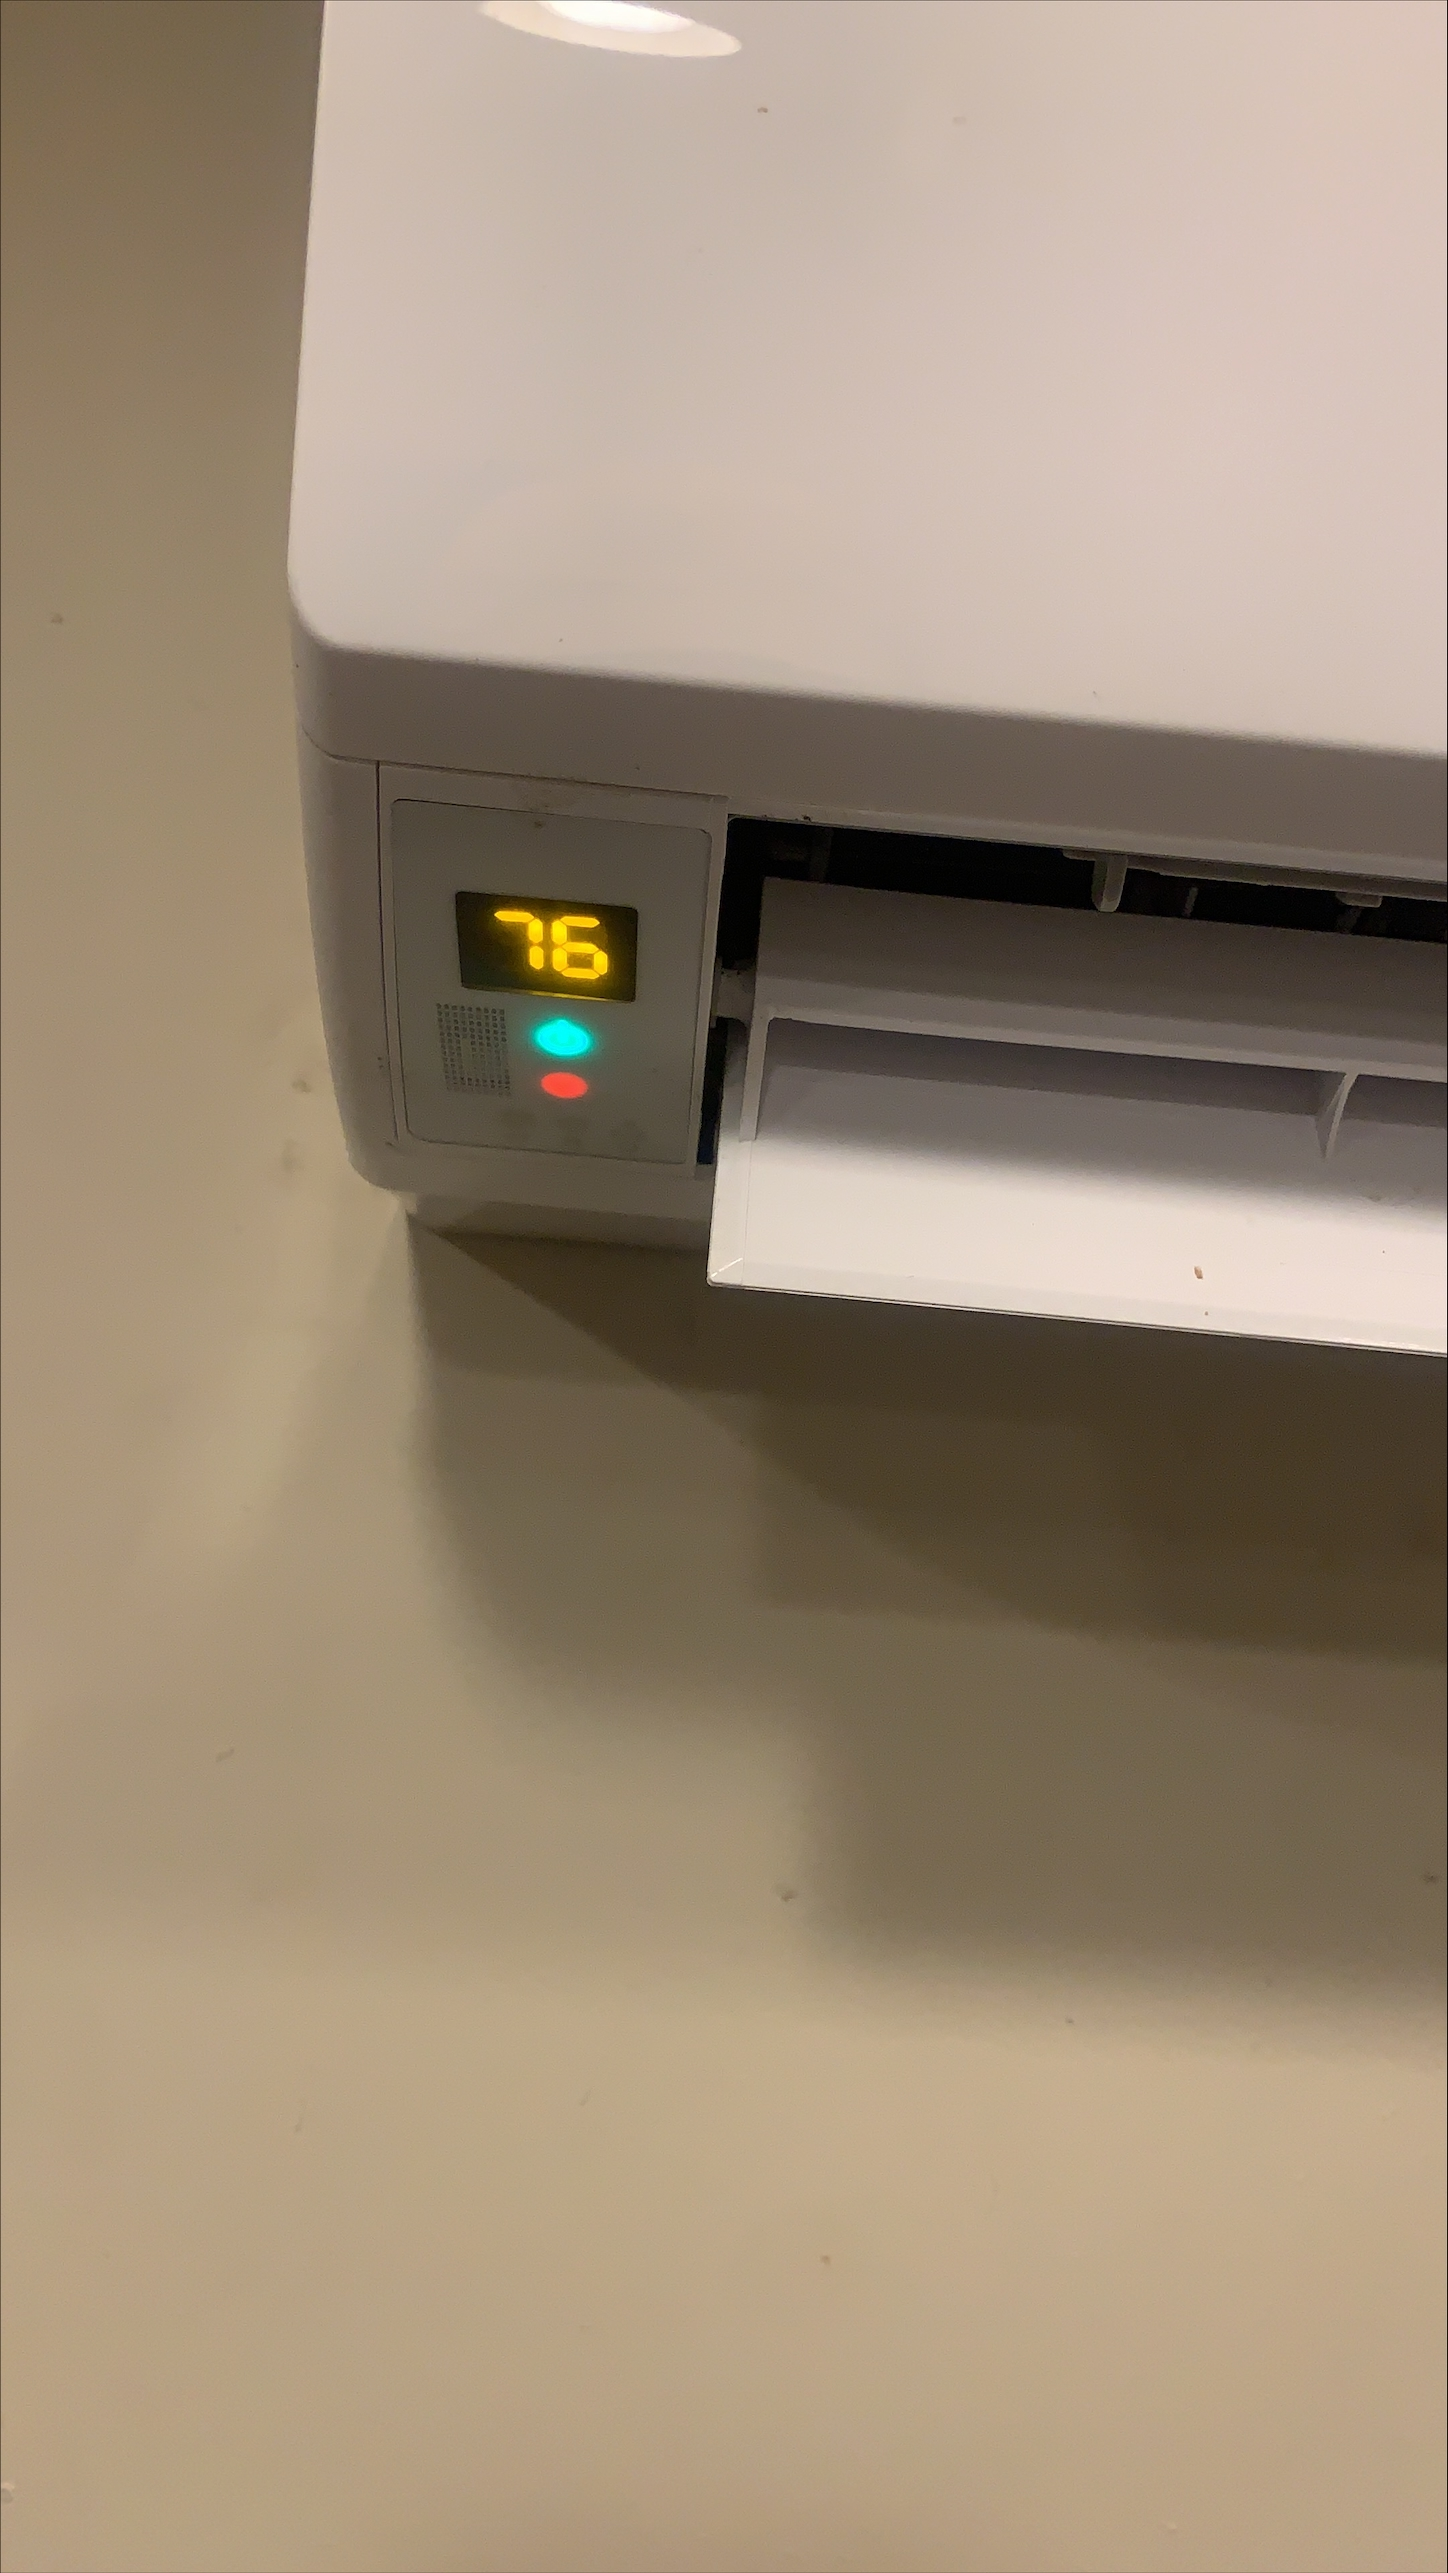
\includegraphics[scale=0.1]{images/ac.png}
		\caption{Caption.}
		\label{fig:ac}
	\end{figure}

	\begin{figure}[htbp!]
		\centering
		\includegraphics[angle=270, scale=0.05]{images/ac_remote.png}
		\caption{Caption.}
		\label{fig:ac_remote}
	\end{figure}

	\begin{figure}[htbp!]
		\centering
		\includegraphics[angle=270, scale=0.05]{images/remote_shutter.png}
		\caption{Caption.}
		\label{fig:remote_shutter}
	\end{figure}

	\begin{figure}[htbp!]
		\centering
		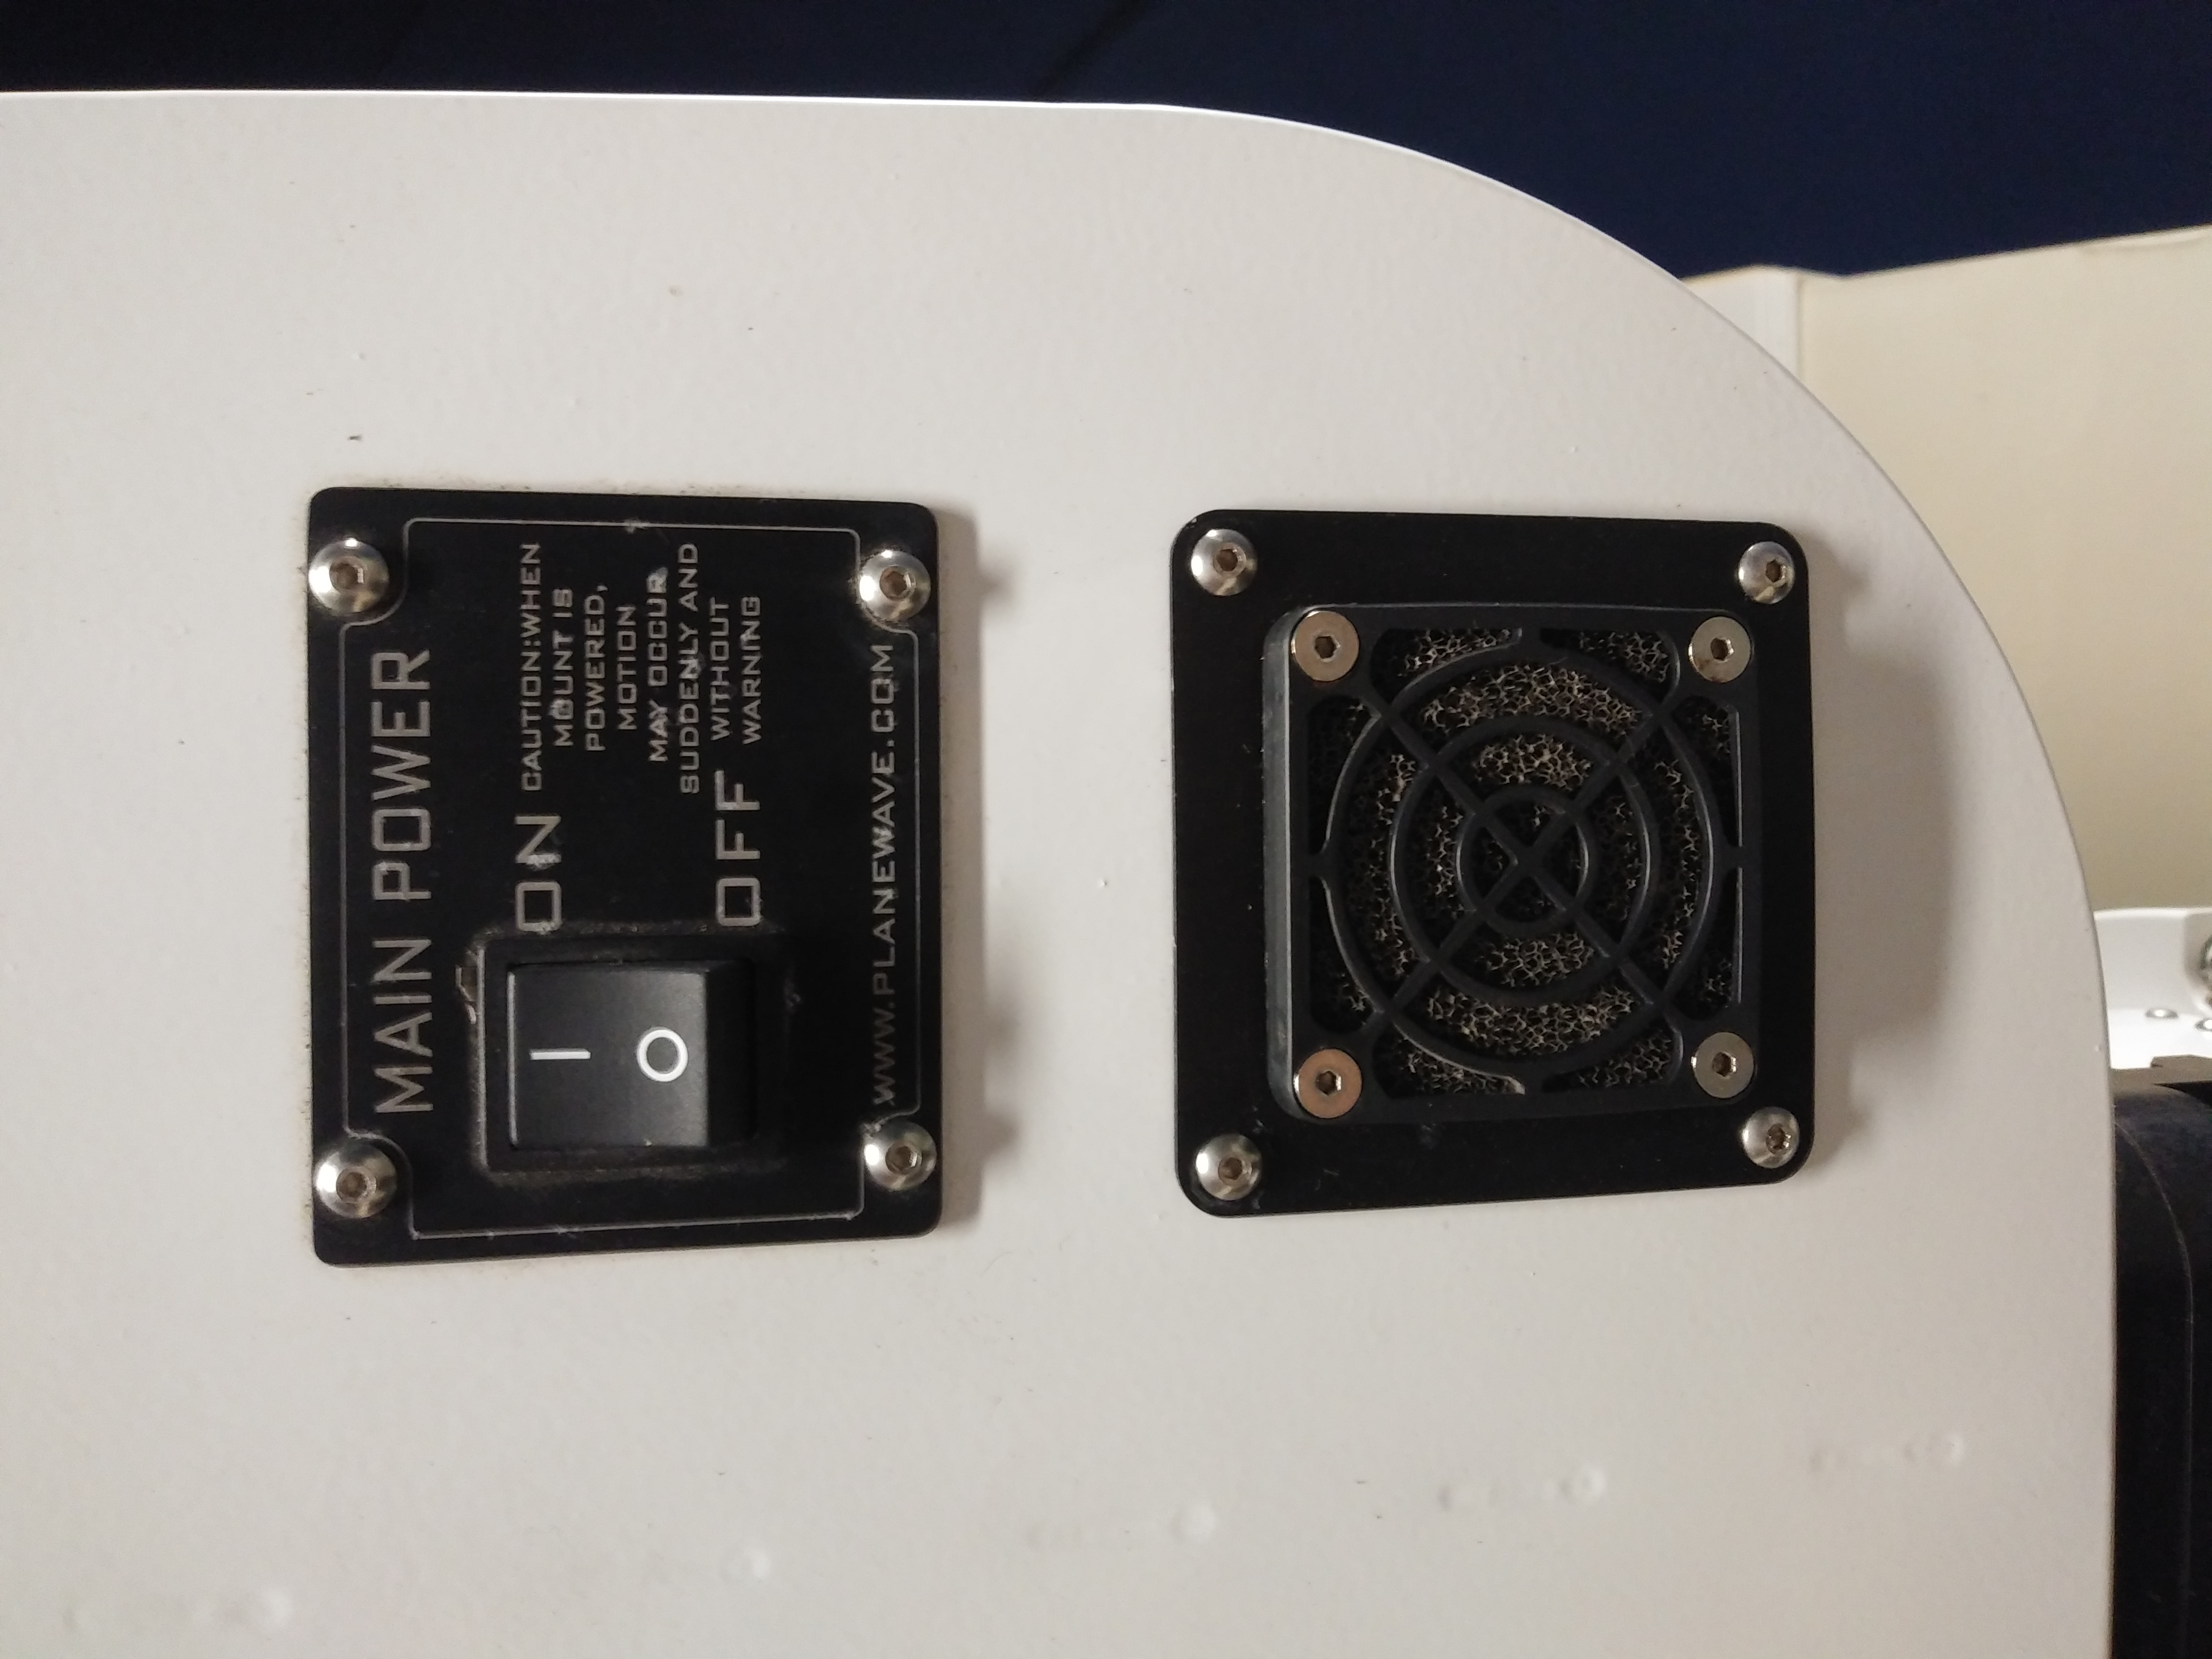
\includegraphics[angle=270, scale=0.05]{images/mount_switch.png}
		\caption{Caption.}
		\label{fig:mount_switch}
	\end{figure}

	\begin{figure}[htbp!]
		\centering
		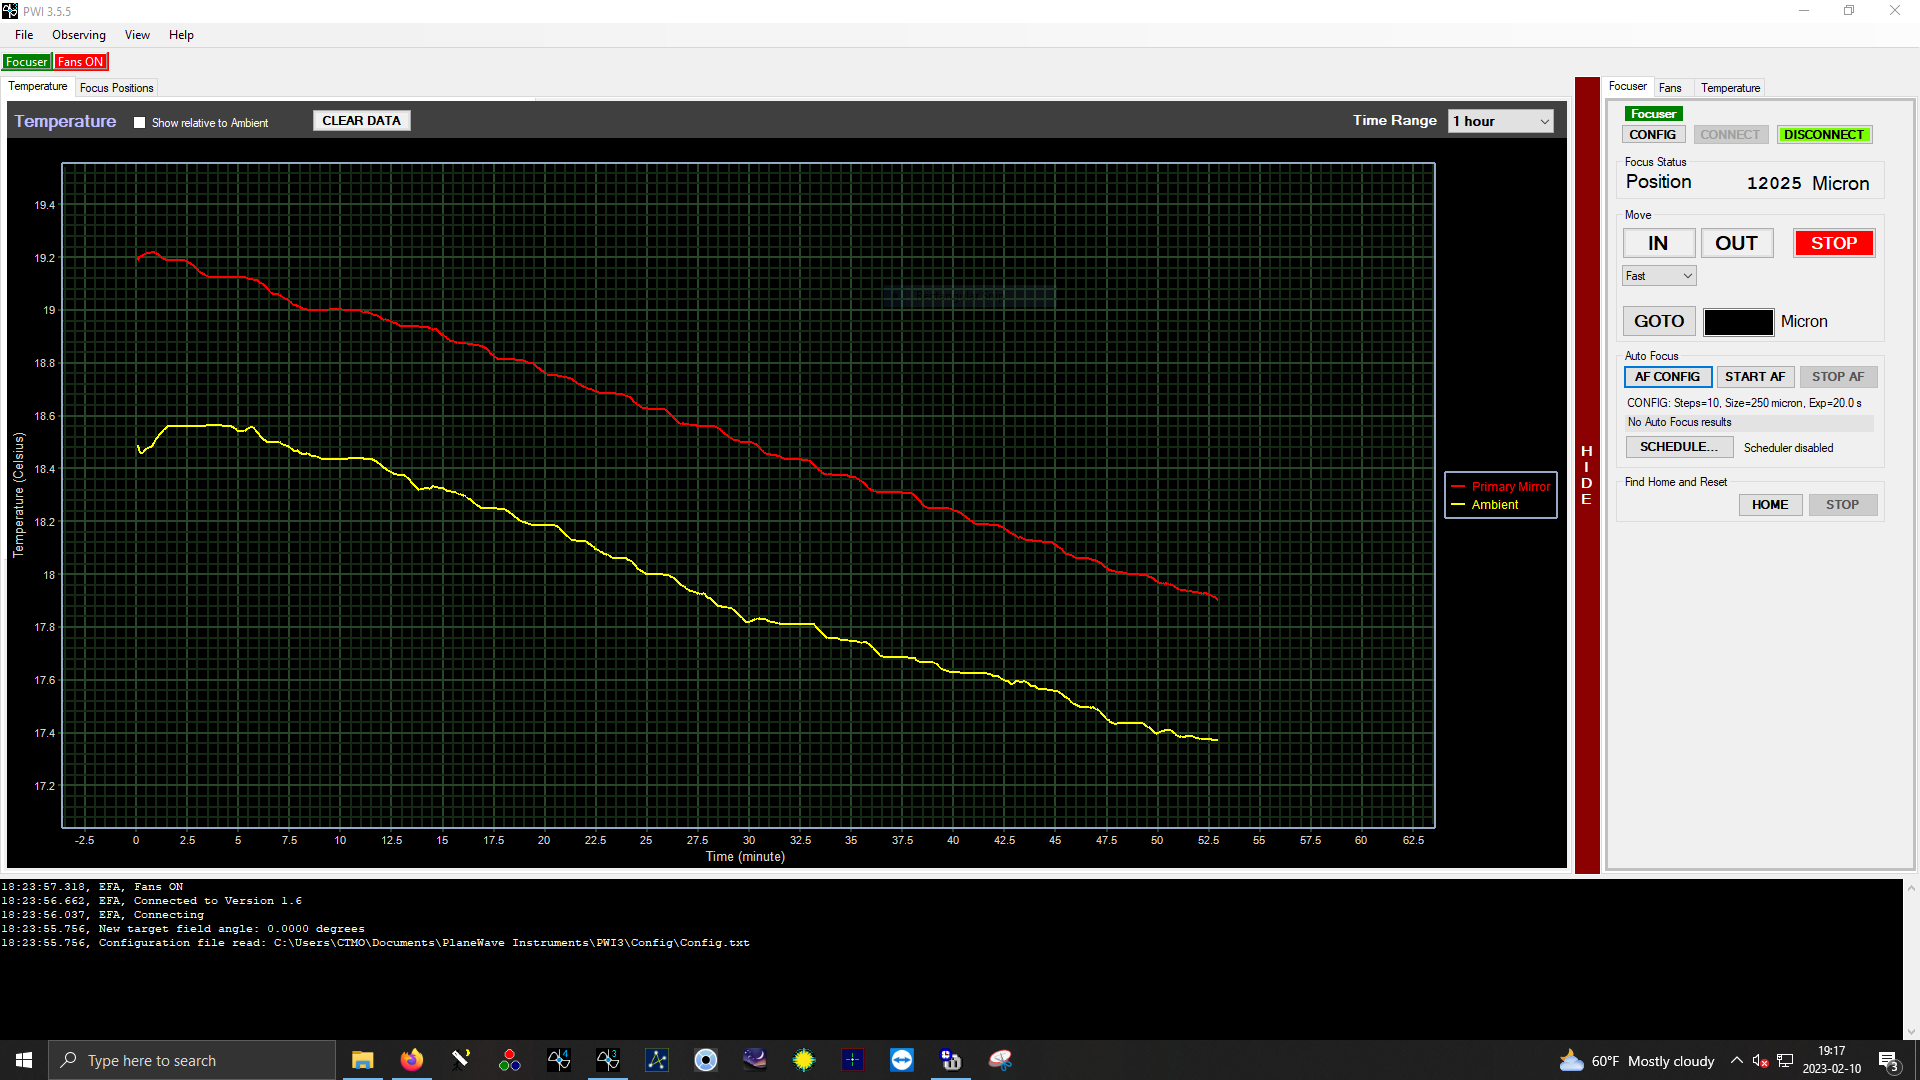
\includegraphics[scale=0.25]{images/pwi3-1.png}
		\caption{Caption.}
		\label{fig:pwi3-1}
	\end{figure}
	
	\begin{figure}[htbp!]
		\centering
		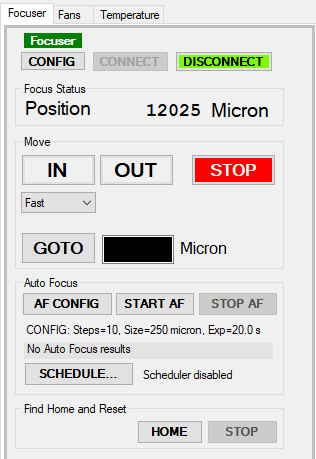
\includegraphics[scale=0.75]{images/pwi3-2.png}
		\caption{Caption.}
		\label{fig:pwi3-2}
	\end{figure}
	
	\begin{figure}[htbp!]
		\centering
		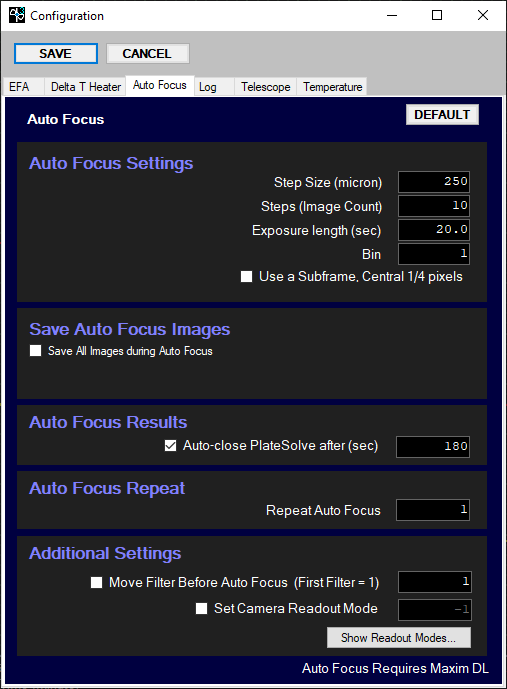
\includegraphics[scale=0.75]{images/pwi3-3.png}
		\caption{Caption.}
		\label{fig:pwi3-4}
	\end{figure}

	\begin{figure}[htbp!]
		\centering
		
\includegraphics[scale=0.25]{images/maxim-1.png}
		\caption{Caption.}
		\label{fig:maxim-1}
	\end{figure}
	
	\begin{figure}[htbp!]
		\centering
		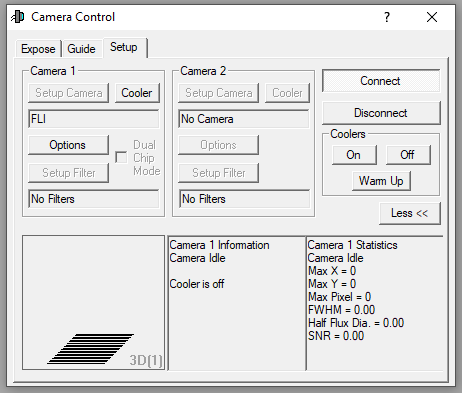
\includegraphics[scale=0.75]{images/maxim-2.png}
		\caption{Caption.}
		\label{fig:maxim-2}
	\end{figure}
	
	\begin{figure}[htbp!]
		\centering
		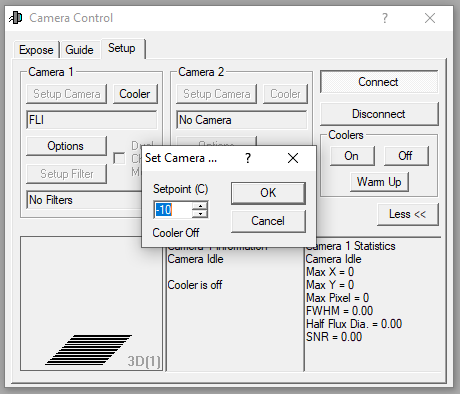
\includegraphics[scale=0.75]{images/maxim-3.png}
		\caption{Caption.}
		\label{fig:maxim-3}
	\end{figure}
	
	\begin{figure}[htbp!]
		\centering
		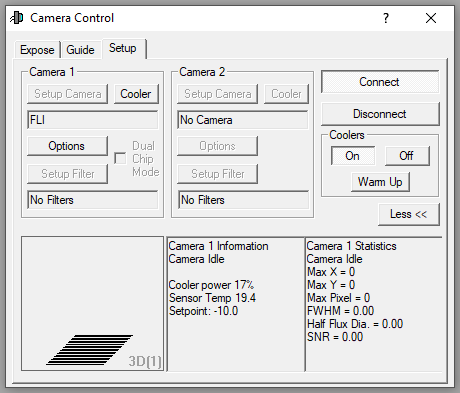
\includegraphics[scale=0.75]{images/maxim-4.png}
		\caption{Caption.}
		\label{fig:maxim-4}
	\end{figure}
	
	\begin{figure}[htbp!]
		\centering
		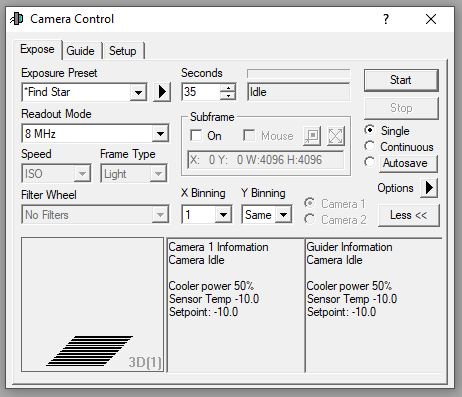
\includegraphics[scale=0.75]{images/maxim-5.png}
		\caption{Caption.}
		\label{fig:maxim-5}
	\end{figure}
	
	\begin{figure}[htbp!]
		\centering
		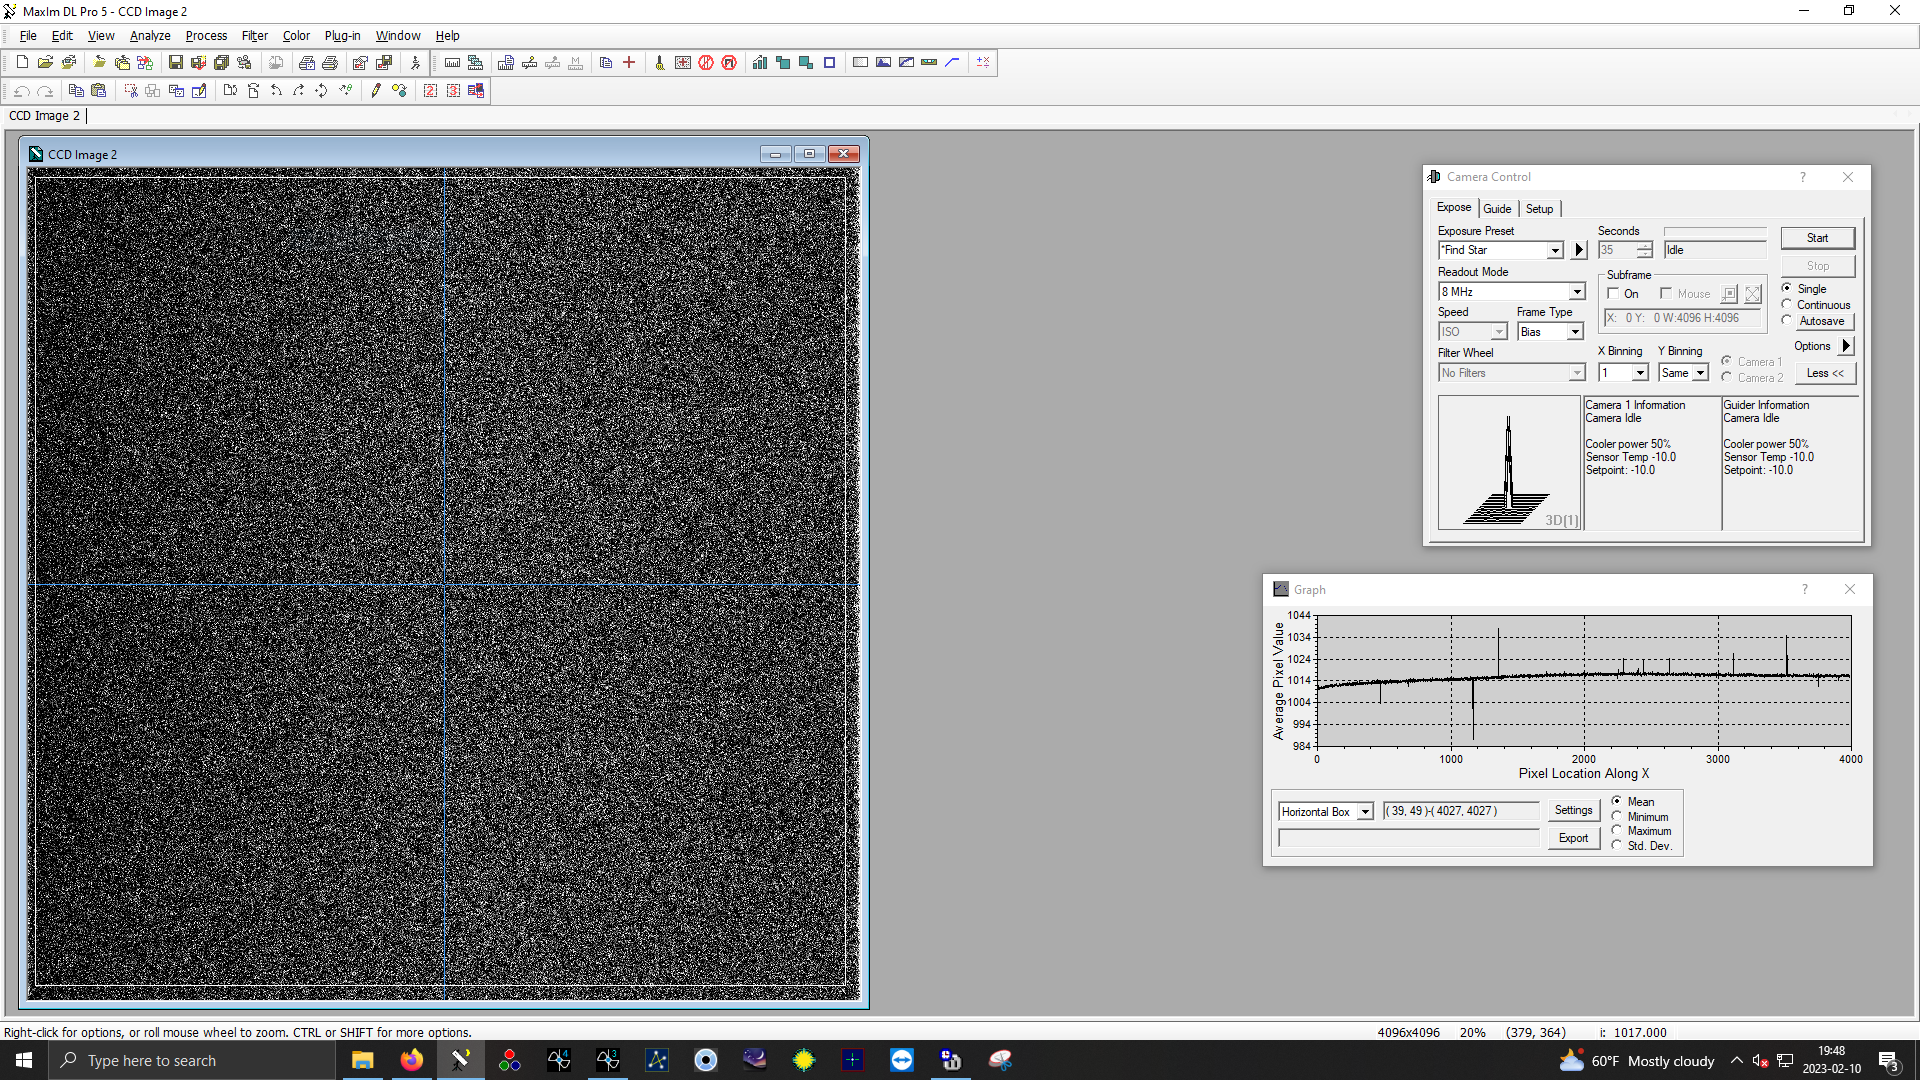
\includegraphics[scale=0.25]{images/maxim-6.png}
		\caption{Caption.}
		\label{fig:maxim-6}
	\end{figure}
	
	\begin{figure}[htbp!]
		\centering
		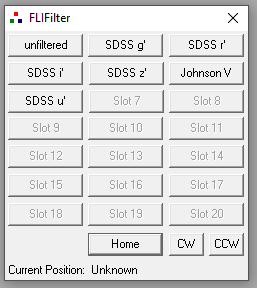
\includegraphics[scale=1]{images/flifilter-1.png}
		\caption{Caption.}
		\label{fig:flifilter-1}
	\end{figure}
	
	\begin{figure}[htbp!]
		\centering
		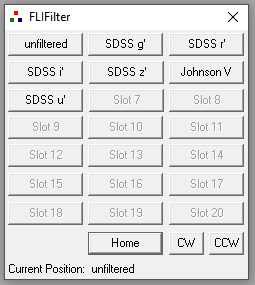
\includegraphics[scale=1]{images/flifilter-2.png}
		\caption{Caption.}
		\label{fig:flifilter-2}
	\end{figure}
	
	\begin{figure}[htbp!]
		\centering
		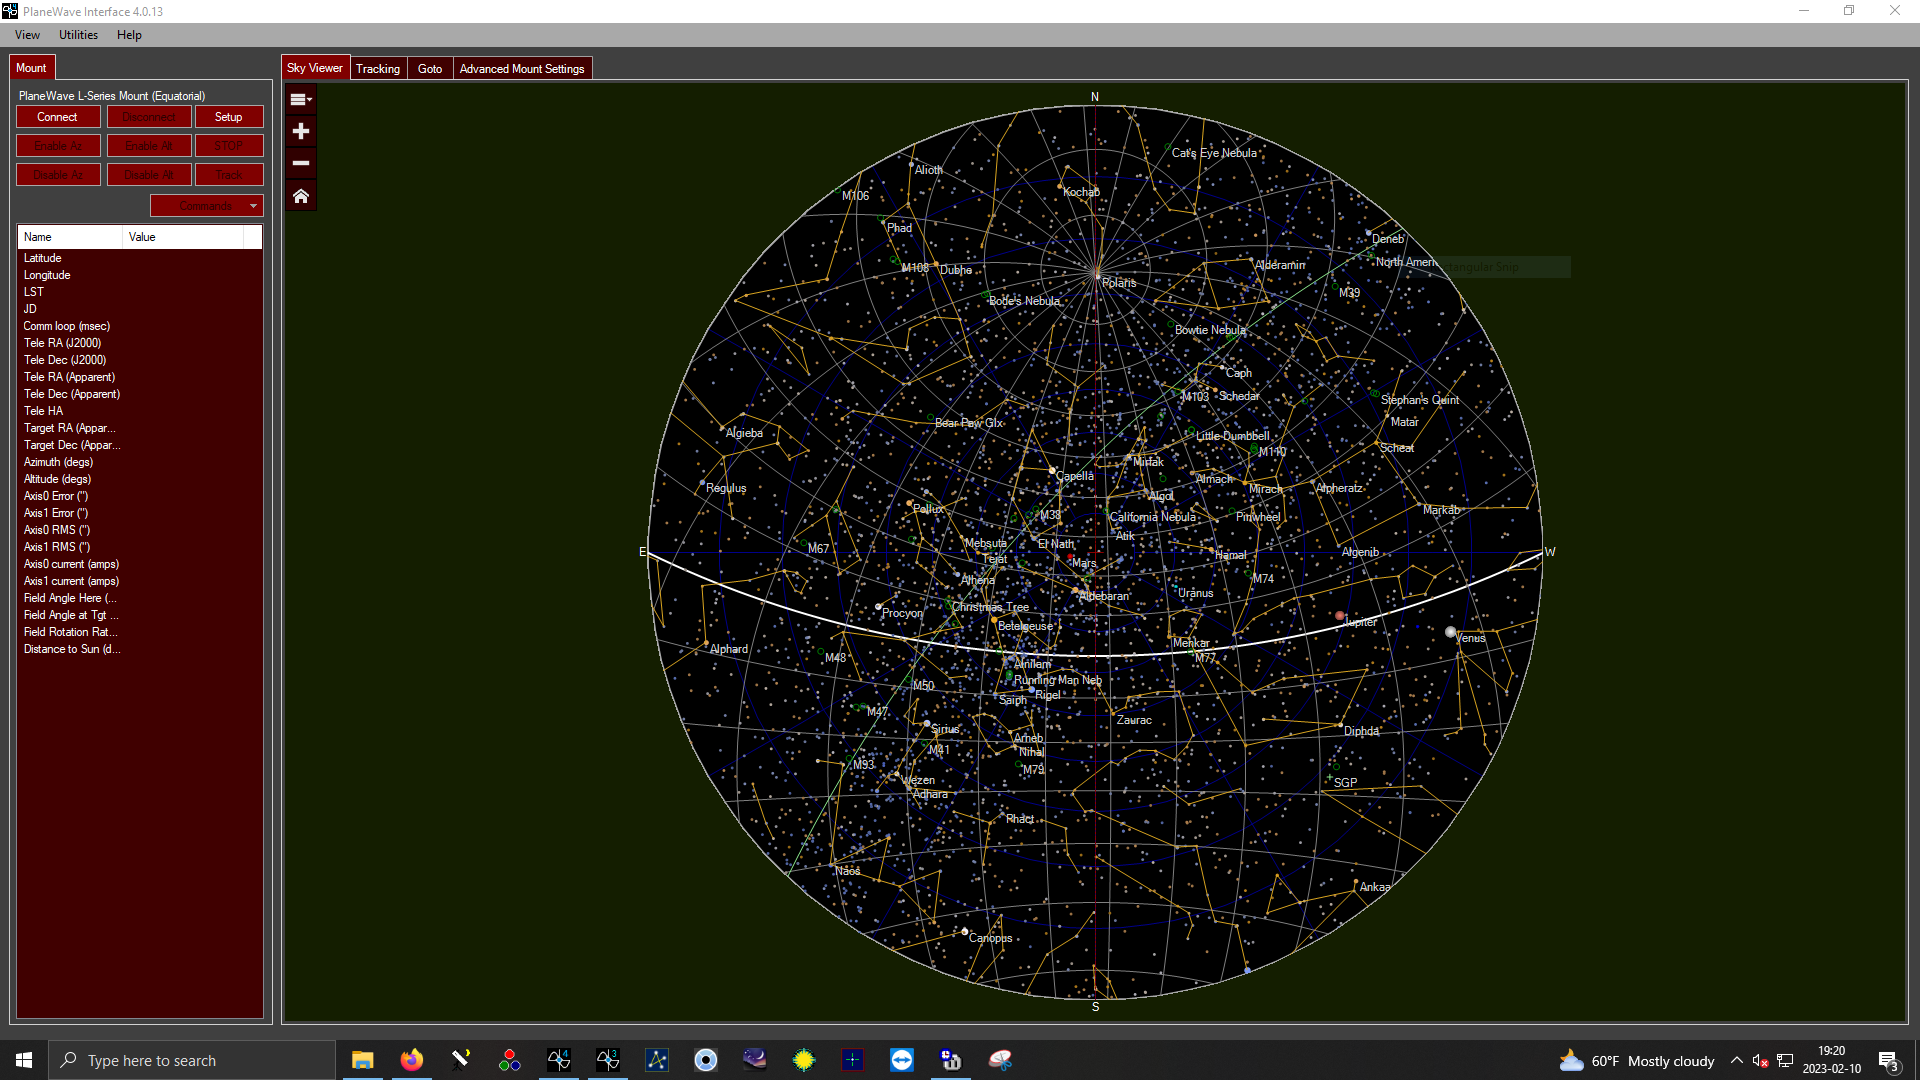
\includegraphics[scale=0.25]{images/pwi4-1.png}
		\caption{Caption.}
		\label{fig:pwi4-1}
	\end{figure}
	
	\begin{figure}[htbp!]
		\centering
		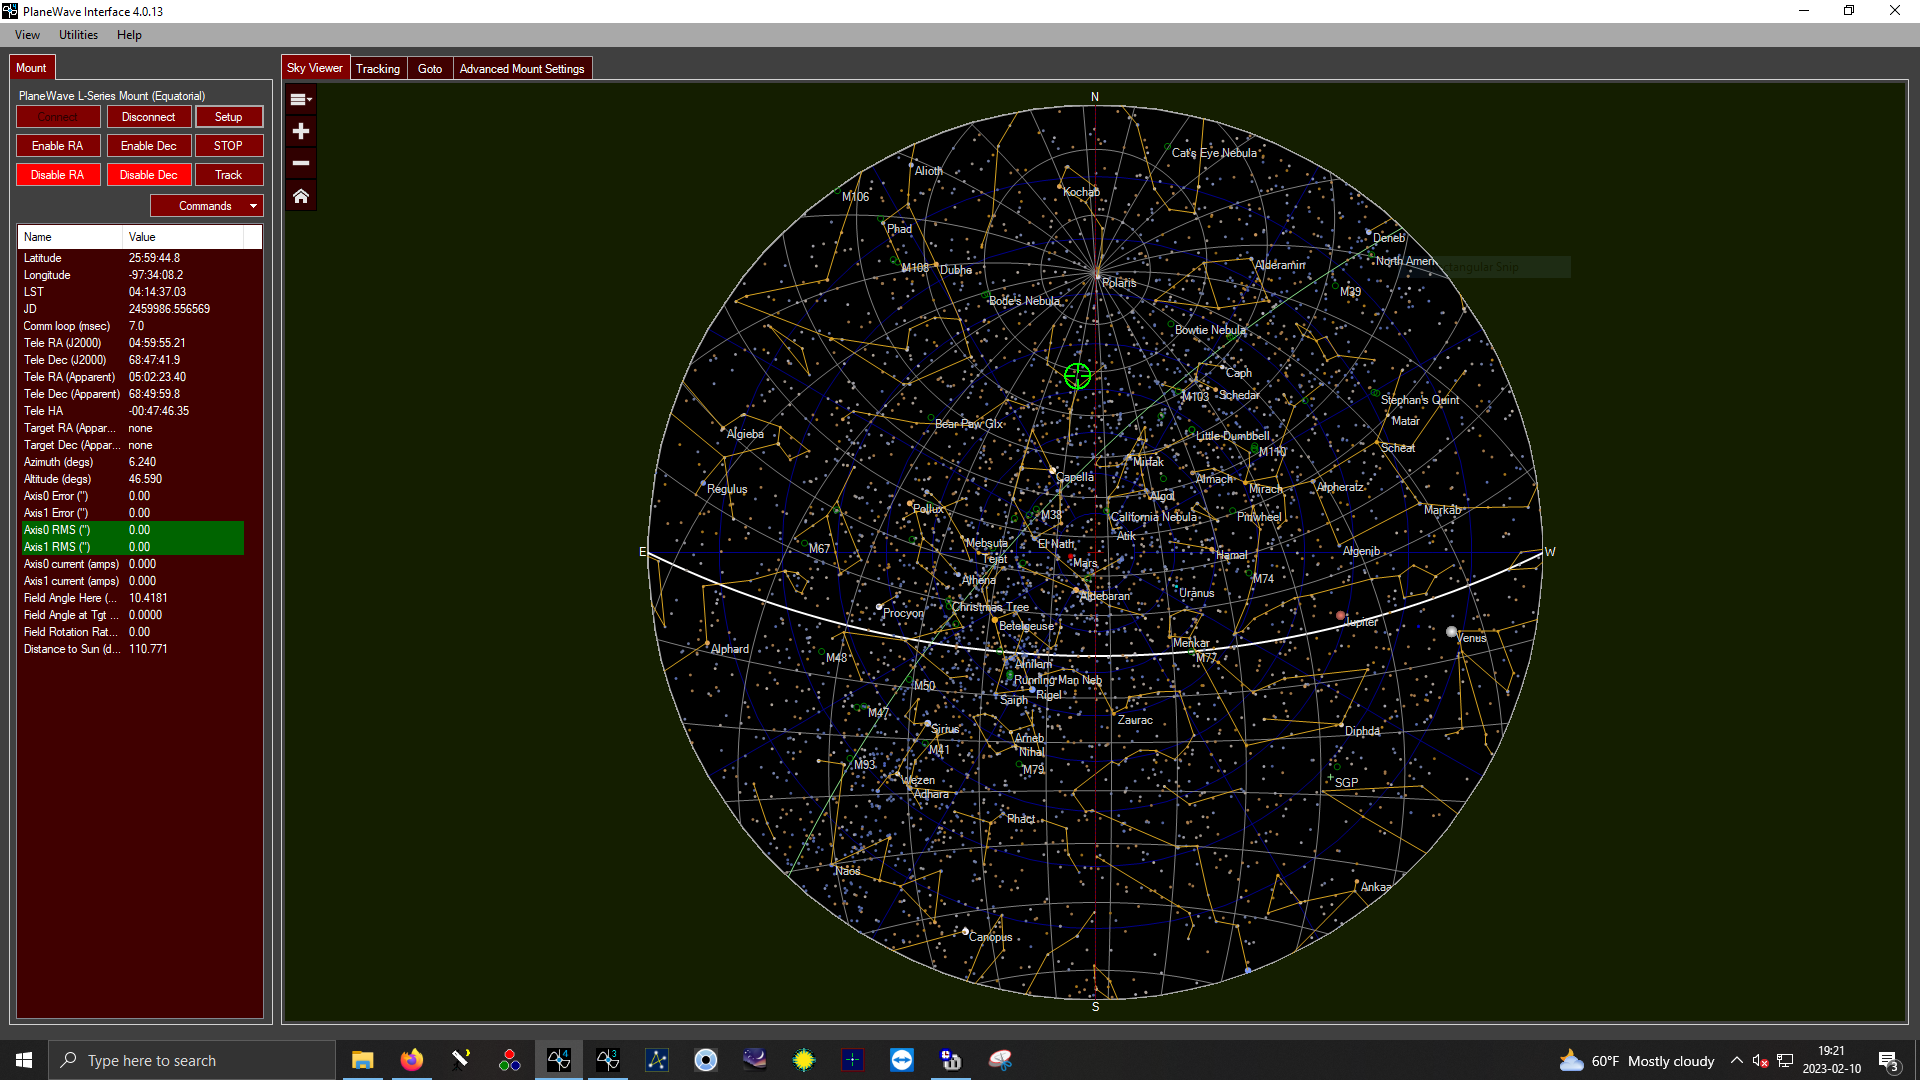
\includegraphics[scale=0.25]{images/pwi4-2.png}
		\caption{Caption.}
		\label{fig:pwi4-2}
	\end{figure}
	
	\begin{figure}[htbp!]
		\centering
		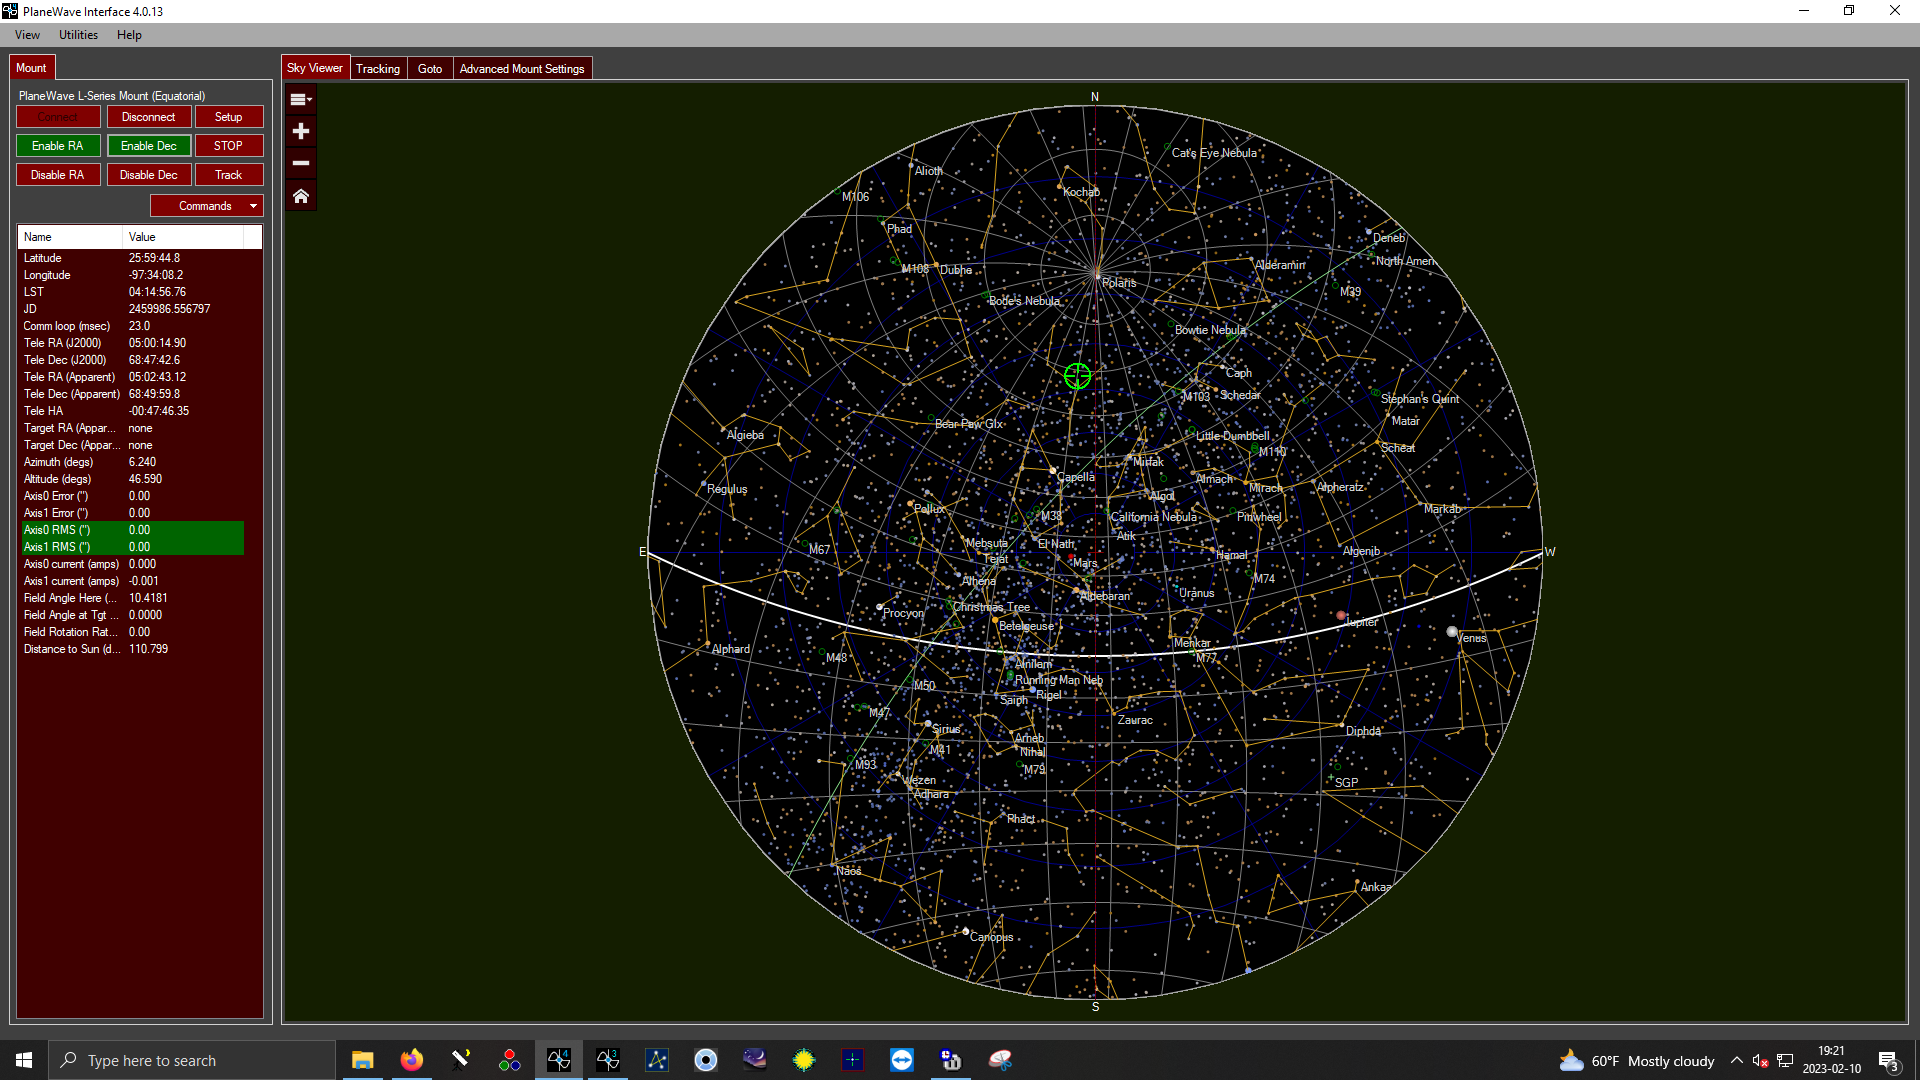
\includegraphics[scale=0.25]{images/pwi4-3.png}
		\caption{Caption.}
		\label{fig:pwi4-3}
	\end{figure}
	
	\begin{figure}[htbp!]
		\centering
		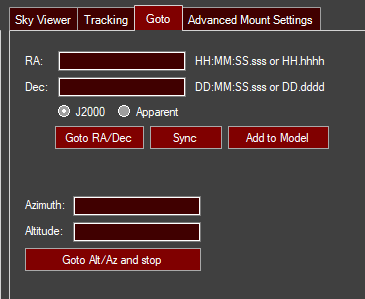
\includegraphics[scale=0.75]{images/pwi4-4.png}
		\caption{Caption.}
		\label{fig:pwi4-4}
	\end{figure}

	\begin{figure}[htbp!]
		\centering
		\includegraphics[angle=270, scale=0.05]{images/remote_dome.png}
		\caption{Caption.}
		\label{fig:remote_dome}
	\end{figure}
	
	\begin{figure}[htbp!]
		\centering
		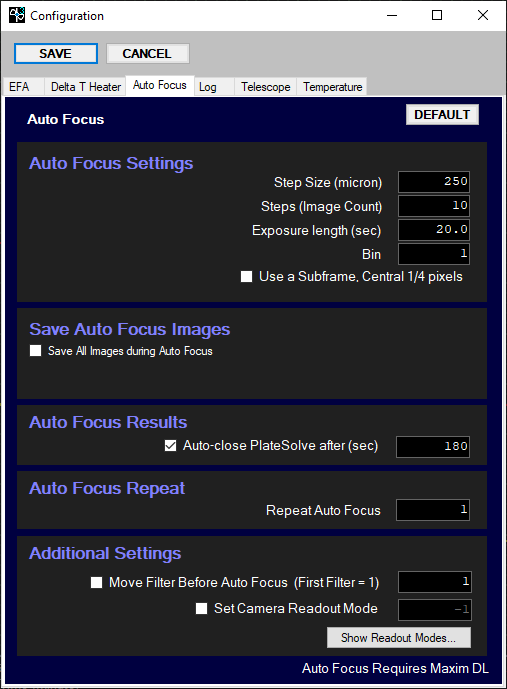
\includegraphics[scale=0.6]{images/pwi3-3.png}
		\caption{Caption.}
		\label{fig:pwi3-3}
	\end{figure}
	
	\begin{figure}[htbp!]
		\centering
		\includegraphics[scale=0.5]{images/ctmo_format.png}
		\caption{The directory structure for CTMO data. The object file names should be a single, unbroken string of the object's name. The (g, 100) and (i, 10) are the filters and exposure time used for that particular object (you don't need to include this in the file name).}
		\label{fig:directory}
	\end{figure}
	
\end{document}